% Sprint-facing short version. The archival paper is main.tex and stays the
% source of truth; this file reorders and demotes, it never restates a result
% differently. Both read the same numbers.tex, so a rebuild moves them together.
%
% Front budget, fixed before the prose was written (6-8 pages):
%   abstract 150w | what we established 0.75p | method 0.75p | results 2p
%   persona 1p | what is new 0.5p | limitations + dual-use 1p
% Everything else is demoted to the appendix and cited from the body.
\documentclass[11pt,a4paper]{article}

\usepackage[a4paper,margin=0.85in]{geometry}
\usepackage{amsmath}
\usepackage{booktabs}
\usepackage{graphicx}
\usepackage[hidelinks]{hyperref}
\usepackage[numbers,sort&compress]{natbib}
\usepackage{array}

\graphicspath{{figs/}}

\newcommand{\armR}{\textbf{R}}
\newcommand{\armNp}{\textbf{N\textsuperscript{+}}}
\newcommand{\armNm}{\textbf{N\textsuperscript{--}}}

% Every measured number resolves through here. Nothing is typed in this file,
% for the same reason nothing is typed in main.tex.
% Generated by scripts/paper_numbers.py. Do not edit.
% Every result in main.tex resolves through these macros.
\newcommand{\NModels}{9}
\newcommand{\NCells}{81}
\newcommand{\NSplits}{5}
\newcommand{\MeanR}{0.906}
\newcommand{\MeanFloor}{0.880}
\newcommand{\MeanResidual}{+0.025}
\newcommand{\NClears}{6}
\newcommand{\NNegative}{2}
\newcommand{\BatterySHA}{342db046213099ad}
\newcommand{\MeanDecisiveR}{41}
\newcommand{\MeanDecisiveN}{4.5}
\newcommand{\MedianDecisiveRatio}{17}
\newcommand{\SmolLMThreeThreeBR}{0.938}
\newcommand{\SmolLMThreeThreeBN}{0.929}
\newcommand{\SmolLMThreeThreeBResid}{+0.009}
\newcommand{\SmolLMThreeThreeBFloor}{0.029}
\newcommand{\QwenThreeFiveNineBR}{0.919}
\newcommand{\QwenThreeFiveNineBN}{0.923}
\newcommand{\QwenThreeFiveNineBResid}{-0.004}
\newcommand{\QwenThreeFiveNineBFloor}{0.010}
\newcommand{\LFMTwoFiveOneTwoBInstructR}{0.905}
\newcommand{\LFMTwoFiveOneTwoBInstructN}{0.858}
\newcommand{\LFMTwoFiveOneTwoBInstructResid}{+0.047}
\newcommand{\LFMTwoFiveOneTwoBInstructFloor}{0.023}
\newcommand{\QwenThreeFiveZeroEightBR}{0.904}
\newcommand{\QwenThreeFiveZeroEightBN}{0.838}
\newcommand{\QwenThreeFiveZeroEightBResid}{+0.067}
\newcommand{\QwenThreeFiveZeroEightBFloor}{0.023}
\newcommand{\QwenThreeFiveFourBR}{0.903}
\newcommand{\QwenThreeFiveFourBN}{0.916}
\newcommand{\QwenThreeFiveFourBResid}{-0.013}
\newcommand{\QwenThreeFiveFourBFloor}{0.015}
\newcommand{\gemmaFourETwoBitR}{0.902}
\newcommand{\gemmaFourETwoBitN}{0.892}
\newcommand{\gemmaFourETwoBitResid}{+0.010}
\newcommand{\gemmaFourETwoBitFloor}{0.007}
\newcommand{\graniteFourOneThreebR}{0.896}
\newcommand{\graniteFourOneThreebN}{0.832}
\newcommand{\graniteFourOneThreebResid}{+0.063}
\newcommand{\graniteFourOneThreebFloor}{0.029}
\newcommand{\QwenThreeFiveTwoBR}{0.895}
\newcommand{\QwenThreeFiveTwoBN}{0.892}
\newcommand{\QwenThreeFiveTwoBResid}{+0.003}
\newcommand{\QwenThreeFiveTwoBFloor}{0.001}
\newcommand{\SmolLMTwoOneSevenBInstructR}{0.890}
\newcommand{\SmolLMTwoOneSevenBInstructN}{0.843}
\newcommand{\SmolLMTwoOneSevenBInstructResid}{+0.047}
\newcommand{\SmolLMTwoOneSevenBInstructFloor}{0.015}
\newcommand{\LadderSmall}{Qwen3.5-0.8B}
\newcommand{\LadderLarge}{Qwen3.5-9B}
\newcommand{\LadderRRise}{+0.014}
\newcommand{\LadderNRise}{+0.085}
\newcommand{\LadderResidFall}{-0.071}
\newcommand{\PooledSizeCorr}{-0.67}
\newcommand{\PooledFloorCorr}{+0.68}
\newcommand{\LadderFamily}{qwen}
\newcommand{\LadderNSizes}{4}
\newcommand{\WithinFamilyCorr}{-0.84}
\newcommand{\OutsideFamilyCorr}{-0.19}
\newcommand{\NOutsideFamily}{5}
\newcommand{\TokensR}{13.2}
\newcommand{\TokensNm}{26.6}
\newcommand{\TokenInflation}{2.0}
\newcommand{\MatchedBandLo}{13}
\newcommand{\MatchedBandHi}{24}
\newcommand{\MatchedResidual}{+0.021}
\newcommand{\RealLengthRule}{0.541}
\newcommand{\RealTiedAcc}{0.899}
\newcommand{\RealDecompFit}{0.904}
\newcommand{\FloorLengthRule}{0.695}
\newcommand{\FloorTiedAcc}{0.848}
\newcommand{\FloorDecompFit}{0.884}
\newcommand{\MostLengthModel}{granite-4.1-3b}
\newcommand{\MostLengthRule}{0.835}
\newcommand{\MostLengthFit}{0.833}
\newcommand{\NMassDrop}{8}
\newcommand{\MedianMassDrop}{+0.011}
\newcommand{\MassDropSignP}{0.039}
\newcommand{\ReasoningModel}{SmolLM3-3B}
\newcommand{\ReasoningMassDrop}{0.193}
\newcommand{\ReasoningResid}{+0.009}
\newcommand{\MassDropExclReasoning}{+0.009}
\newcommand{\ResidShiftAnswered}{+0.002}
\newcommand{\PersonaSignCorrect}{20}
\newcommand{\PersonaSignTotal}{20}
\newcommand{\PersonaSepReal}{+0.791}
\newcommand{\PersonaSepInvented}{+0.781}
\newcommand{\PersonaExcess}{+0.133}
\newcommand{\PersonaNonsenseShare}{66}
\newcommand{\PersonaNRetain}{2}
\newcommand{\PersonaNModelsTested}{5}
\newcommand{\PersonaRetainTop}{Qwen3.5-9B}
\newcommand{\PersonaRetainTopVal}{+0.415}
\newcommand{\DetKeptAuroc}{0.596}
\newcommand{\DetKeptTPR}{0}
\newcommand{\DetBestName}{answer mass}
\newcommand{\DetBestAuroc}{0.821}
\newcommand{\DetBestTPR}{40}
\newcommand{\DetFPR}{5}
\newcommand{\DetNModels}{9}
\newcommand{\DetBestModel}{Qwen3.5-2B}
\newcommand{\DetBestModelAuroc}{1.000}
\newcommand{\StatedNModels}{5}
\newcommand{\StatedNResponsive}{4}
\newcommand{\StatedNItems}{12}
\newcommand{\StatedHaveLo}{0.869}
\newcommand{\StatedHaveHi}{1.000}
\newcommand{\StatedHideLo}{0.901}
\newcommand{\StatedHideHi}{1.000}
\newcommand{\StatedFakeLo}{0.947}
\newcommand{\StatedFakeHi}{0.999}
\newcommand{\StatedBaseLo}{0.246}
\newcommand{\StatedBaseHi}{0.491}
\newcommand{\StatedInertModel}{LFM2.5-1.2B-Instruct}
\newcommand{\StatedInertLo}{0.500}
\newcommand{\StatedInertHi}{0.547}
\newcommand{\StatedInertBase}{0.491}
\newcommand{\StatedNScored}{24}
\newcommand{\StatedWorstModel}{gemma-4-E2B-it}
\newcommand{\StatedWorstCond}{verbal}
\newcommand{\StatedWorstScored}{16}
\newcommand{\StatedWorstMass}{0.67}
\newcommand{\RevNModels}{5}
\newcommand{\RevNTriad}{3}
\newcommand{\RevNInterp}{2}
\newcommand{\RevSpecMargin}{0.30}
\newcommand{\RevGapLo}{+0.054}
\newcommand{\RevGapHi}{+0.059}
\newcommand{\RevSpecLo}{+0.88}
\newcommand{\RevSpecHi}{+1.40}
\newcommand{\RevInertModel}{LFM2.5-1.2B-Instruct}
\newcommand{\RevInertMargin}{+0.116}
\newcommand{\RevInertGap}{-0.041}
\newcommand{\RevDropModel}{gemma-4-E2B-it}
\newcommand{\RevDropPairs}{224}
\newcommand{\RevKeptPairs}{4776}
\newcommand{\RevNInvented}{1}
\newcommand{\RevInventedModel}{Qwen3.5-2B}
\newcommand{\RevInventedConcealed}{+0.890}
\newcommand{\RevInventedVerbal}{+0.635}
\newcommand{\RevInventedGap}{+0.255}
\newcommand{\NeutModel}{Qwen3.5-2B}
\newcommand{\NeutResidBinary}{+0.006}
\newcommand{\NeutResidNeutral}{+0.006}
\newcommand{\NeutFloorShift}{+0.003}
\newcommand{\NeutCohRealBin}{0.896}
\newcommand{\NeutCohRealNeut}{0.898}
\newcommand{\NeutPCReal}{0.316}
\newcommand{\NeutPCPctReal}{32}
\newcommand{\NeutMajReal}{3}
\newcommand{\NeutCohInvBin}{0.889}
\newcommand{\NeutCohInvNeut}{0.892}
\newcommand{\NeutPCInv}{0.638}
\newcommand{\NeutPCPctInv}{64}
\newcommand{\NeutMajInv}{90}
\newcommand{\NPersonaCells}{20}
\newcommand{\NPersonaModels}{5}
\newcommand{\PersonaAbovePointThree}{18}
\newcommand{\PersonaMax}{+0.85}
\newcommand{\PersonaMin}{-0.66}
\newcommand{\DepthSpread}{0.109}
\newcommand{\PersonaSpread}{0.276}


\title{\textbf{Does the Persona Change the Preference,\\ or Only the Prose?}\\[.4em]
\large Replace every outcome with invented words and a model's preferences
barely move,\\ so the coherence number cannot be evidence that the model means
them.}

\author{Martin Kaiser \and Gellért Bodorkós\\
\small Apart Research Digital Minds Sprint}

\date{17 August 2026}

\begin{document}
\maketitle

\begin{abstract}
\noindent
Preference-coherence fits a Thurstonian model to a model's pairwise choices and
reads high held-out accuracy as evidence of emergent values. We add the missing
control: the same battery with every referent replaced by an invented word,
holding the prompt, pair set, fit and metric fixed. On
\NModels{} open-weight models at \NDesignReps{} design seeds each, coherence is
\MeanFloor{} on outcomes that refer to nothing against \MeanR{} on real ones ---
a residual of \MeanResidual{}, and \NFailsFloor{} of \NModels{} models do not
clear their own replicate floor. The metric keeps only choice direction:
conviction collapses \MedianDecisiveRatio$\times$ on nonsense while
direction accuracy barely moves. A discarded channel of the same forward pass
separates the arms at AUROC \DetBestAuroc{} against
\DetKeptAuroc{} for the channel coherence keeps. Installed personas still
displace real outcomes further than invented ones, so the instrument is not
blunt. The metric is not broken. It is unanchored.
\end{abstract}

\section{What we established}

\textbf{A coherence score of \MeanR{} survives the removal of all meaning,
falling only to \MeanFloor{}.} We built the null arm that preference-coherence
work has not had --- the same outcomes with invented referents --- and ran it as
a measurement rather than a demonstration: \NModels{} models across
\NFamilies{} families, \NCells{} cells, \NSplits{} splits and \NDesignReps{}
independent design replicates per cell, every cell scored against its own
replicate noise floor. The result is a card, not a headline.

\textbf{Three findings, in the order we would defend them.} The mechanism is
firm: thresholding a preference to a hard label keeps direction and discards
strength, so a model that is uniformly near-indifferent about gibberish scores
as coherent about it (\S\ref{sec:mech}). The dissociation is firm: the
information the metric throws away separates real from invented outcomes far
better than the information it keeps (\S\ref{sec:det}). The headline residual is
marginal and we report it as such --- \MeanResidual{}, bootstrap 95\% CI
[\ResidCiLo, \ResidCiHi], \NPositiveModels{} of \NModels{} positive at a
sign-test $p$ of \ResidSignP{} (\S\ref{sec:resid}). That the residual is small
\emph{is} the claim; it is not a caveat on one.

\textbf{The instrument is not simply blunt, which is what makes the flat result
mean something.} An installed persona displaces real outcomes substantially
further than invented ones in \PersonaAbovePointThree{} of \NPersonaCells{}
conditions (\S\ref{sec:persona}), so the pipeline does register a real change of
preference when one is induced. A metric that could not detect anything would
explain the flatness away.

\textbf{The practical recommendation is one line.} Any claim that a coherence
number reflects values should carry the same number computed on outcomes that
mean nothing. That arm cost one battery and a few dollars of compute.

\section{Method}\label{sec:method}

\textbf{Three arms, differing in exactly one property each.} \armR{} is the real
battery; \armNp{} replaces every referent with an invented word but keeps the
magnitudes; \armNm{} removes the magnitudes too. The prompt, the pair set, the
fit, the split scheme and the metric are held fixed across arms, so
$\armR \to \armNp$ isolates the referent and $\armNp \to \armNm$ the arithmetic.
Choices are read from the first-token logit distribution rather than sampled,
which removes temperature and seed from the design and restricts the study to
models that expose logprobs.

\textbf{Every cell is scored against its own noise floor, not against zero.} A
design replicate redraws the outcome subsample and the pair set under a new
seed; the spread of a cell across \NDesignReps{} such replicates is that cell's
design noise floor. A residual smaller than that floor is not a finding about
the model, and we say so per model rather than in aggregate. \NHosted{} larger
models reached over a hosted API are reported \emph{beside} the ladder and never
inside its mean: different serving stack, different harness hash
(Appendix~\ref{app:figs}).

\textbf{Provenance.} Predictions were registered before the first model ran, the
battery is hash-pinned (\texttt{\BatterySHA\ldots}), and every measured number
in this document is emitted from the results card by
\texttt{scripts/paper\_numbers.py} rather than typed. The pipeline end to end is
Appendix Figure~\ref{fig:pipeline}; the claims ledger
(\NClaimsEstablished{} established, \NClaimsProvisional{} provisional) is
Appendix Table~\ref{tab:claims}.

\textbf{What this document leaves out.} Two tracks run in the archival paper and
not here: what models \emph{say} about a disposition they were given
(Appendix Table~\ref{tab:stated}), and whether an instruction to conceal a
disposition changes what they choose as well as what they say
(Appendix Table~\ref{tab:revealed}, with directive compliance in
Table~\ref{tab:comply}). They are secondary to the claim above and are reported
in full rather than summarised here.

\section{Results}

\subsection{The metric barely separates real outcomes from meaningless ones}
\label{sec:resid}

\textbf{Coherence averages \MeanR{} on real outcomes and \MeanFloor{} on
invented ones, a residual of \MeanResidualPrecise{}.} Table~\ref{tab:main} gives
it per model against each model's own floor. \NClears{} of \NModels{} clear that
floor, \NFailsFloor{} do not, and \NNegative{} of those \NFailsFloor{} score
higher on invented outcomes than on real ones. The across-model standard
deviation (\ResidSD) is larger than the mean.

\textbf{The \NClears{} clears are two different things, and only
\NClearsConviction{} are the effect this paper is about.} Those three commit on
real outcomes and go near-indifferent on invented ones. The other
\NClearsFlat{}, daggered in Table~\ref{tab:main}, are decisive on under
\FlatDecisiveThreshPct\% of pairs on \emph{both} arms: they clear by being
uniformly near-indifferent, which is not a value system losing its grip.

\textbf{The residual is the referent step alone.} Splitting it at the middle
arm, replacing the referents costs \MeanReferent{} while removing the magnitudes
on top of that costs \MeanArith{} (SD \ArithSD{}, \NArithPositive{} of
\ArmNPlusModels{} positive). On this battery the arithmetic carries none of the
effect, and a study varying only the numbers would have measured nothing.

\textbf{Within the one family that has a ladder, the residual falls as models
grow} --- \LadderResidFall{} across \LadderNSizes{} sizes, because the floor
rises with scale faster than the signal does (Appendix
Figure~\ref{fig:scale}). It does not survive pooling across families, so this is
a within-family statement and not a scaling law.

\begin{table}[tb]
\centering
\caption{\textbf{Per-model results against each model's own noise floor.}
\armR{}, \armNp{}, \armNm{} are held-out accuracy on real outcomes, invented
outcomes with magnitudes kept, and invented outcomes with magnitudes removed,
over \NSplits{} splits and \NDesignReps{} design replicates. \textbf{floor} is
the spread of the same cell across those replicates; \textbf{clears} reports
whether the residual exceeds it and by what factor. $^{*}$ marks a floor too
near zero for a ratio to mean anything; $^{\dagger}$ marks a model decisive on
under \FlatDecisiveThreshPct\% of pairs on both arms. \textbf{dec.} is the share
of pairs at $p<0.2$ or $p>0.8$. Full model ids in
Appendix~\ref{app:tables}.}
\label{tab:main}
\footnotesize
\setlength{\tabcolsep}{4.5pt}
% Generated by scripts/paper_numbers.py. Do not edit.
\begin{tabular}{@{}lrrrrrlrr@{}}
\toprule
model & R & N\textsuperscript{+} & N\textsuperscript{--} & R$-$N\textsuperscript{--} & floor & clears & dec.\ R & dec.\ N\textsuperscript{--} \\
\midrule
\texttt{SmolLM3-3B} & 0.938 & 0.922 & 0.929 & +0.009 & 0.029 & no & 48.7\% & 4.6\% \\
\texttt{Qwen3.5-9B} & 0.919 & 0.920 & 0.923 & -0.004 & 0.010 & no & 45.7\% & 2.7\% \\
\texttt{LFM2.5-1.2B-Instruct} & 0.905 & 0.830 & 0.858 & +0.047 & 0.023 & 2.0$\times$$^{\dagger}$ & 0.1\% & 0.0\% \\
\texttt{Qwen3.5-0.8B} & 0.904 & 0.853 & 0.838 & +0.067 & 0.023 & 2.9$\times$$^{\dagger}$ & 0.1\% & 0.0\% \\
\texttt{Qwen3.5-4B} & 0.903 & 0.921 & 0.916 & -0.013 & 0.015 & no & 33.8\% & 1.9\% \\
\texttt{gemma-4-E2B-it} & 0.902 & 0.899 & 0.892 & +0.010 & 0.007 & 1.5$\times$ & 56.4\% & 2.8\% \\
\texttt{granite-4.1-3b} & 0.896 & 0.836 & 0.832 & +0.063 & 0.029 & 2.2$\times$ & 49.7\% & 14.9\% \\
\texttt{Qwen3.5-2B} & 0.895 & 0.902 & 0.892 & +0.003 & 0.001 & $>$\,floor$^{*}$ & 12.8\% & 0.0\% \\
\texttt{SmolLM2-1.7B-Instruct} & 0.890 & 0.841 & 0.843 & +0.047 & 0.015 & 3.0$\times$$^{\dagger}$ & 0.0\% & 0.0\% \\
\bottomrule
\end{tabular}

\end{table}

\subsection{Direction survives, strength does not}\label{sec:mech}

\textbf{This is the whole mechanism: coherence records which way a model leans
and never how much.} A pair at $p = 0.51$ counts exactly as a pair at
$p = 0.99$. On real outcomes the \NDecisiveModels{} models that commit anywhere
at all commit on \MeanDecisiveR\% of pairs; on invented outcomes the same six
commit on \MeanDecisiveN\% --- a median collapse of
\MedianDecisiveRatio$\times$ --- while direction accuracy barely moves
(Figure~\ref{fig:strength}). A model almost perfectly indifferent about
gibberish, but \emph{consistently} so, scores as coherent about it. This is a
property of the metric, not a failure of the fit.

\begin{figure}[tb]
\centering
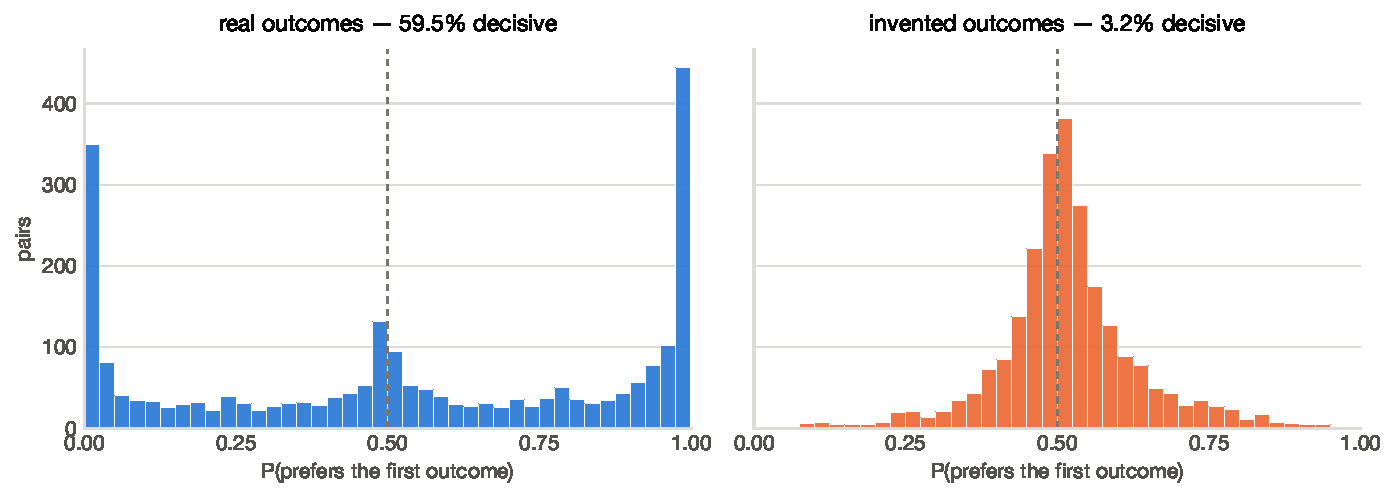
\includegraphics[width=.80\textwidth]{fig3_strength.pdf}
\caption{\textbf{On real outcomes preference mass moves to the edges; on
invented outcomes it piles up at indifference.} Coherence reads only which side
of $0.5$ each pair falls on, so both distributions score alike. The same story
appears as trajectories in Appendix Figure~\ref{fig:state}.}
\label{fig:strength}
\end{figure}

\subsection{The model can tell. The metric does not look.}\label{sec:det}

\textbf{A channel of the same forward pass that coherence discards separates
real from invented outcomes at AUROC \DetBestAuroc{}, against \DetKeptAuroc{}
for the channel coherence keeps.} Every pair was run in both arms, so for one
model and one pair index there are two forward passes differing only in whether
the outcomes refer to anything --- verified-clean negatives and verified
positives, matched by construction rather than by selection
(Figure~\ref{fig:detector}). Thresholding to a hard label discards magnitude and
renormalising over the two options discards the mass placed on neither; those
are precisely the quantities the hallucination-detection literature reads
\citep{farquhar2024semantic,kossen2024sep}. The information is in the forward
pass. The metric declines to look at it.

\textbf{This is an oracle bound, not a deployable detector.} The arm labels are
in hand, so \DetBestAuroc{} is an upper bound on what such a channel could do
without them; we report detection at a \DetFPR\% false-positive rate calibrated
on real-outcome rows alone (\DetBestTPR\%), never a threshold chosen by looking
at the nonsense.

\begin{figure}[tb]
\centering
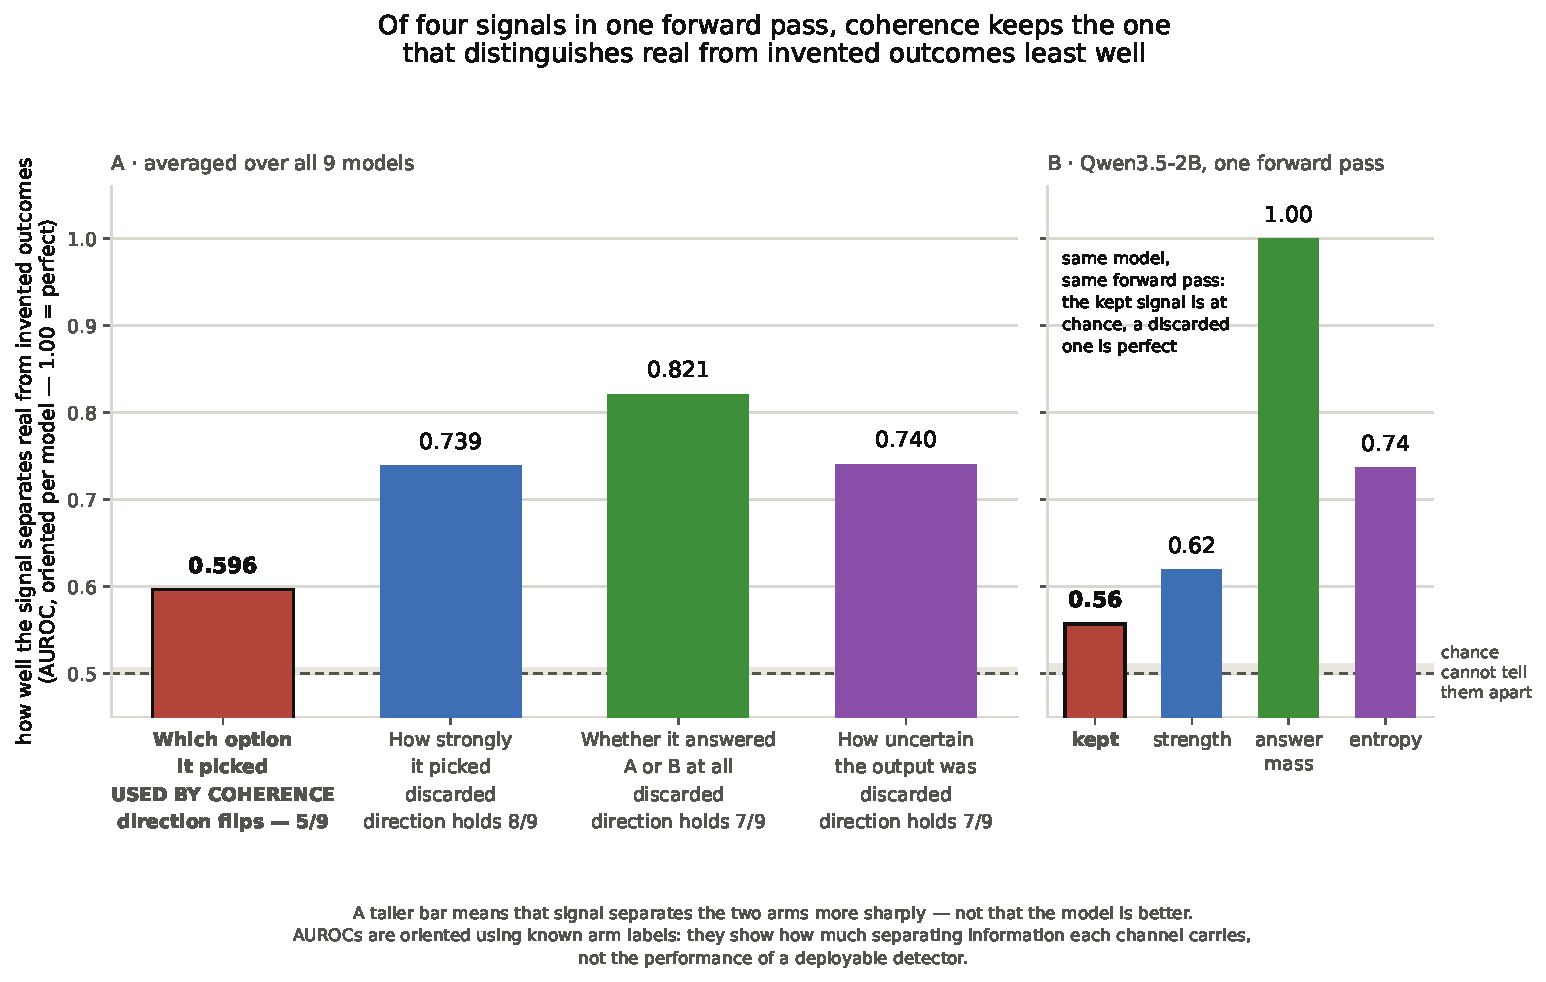
\includegraphics[width=.80\textwidth]{fig4_detector.pdf}
\caption{\textbf{The discarded channel separates the arms; the kept channel does
not.} Per-model separation for each channel of one forward pass. Arm labels are
in hand, so these are oracle upper bounds and are labelled as such.}
\label{fig:detector}
\end{figure}

\section{The instrument is not blunt: personas move wanting, not only prose}
\label{sec:persona}

\textbf{An installed persona displaces real outcomes far more than invented ones
in \PersonaAbovePointThree{} of \NPersonaCells{} conditions.} We install a
dispositional trait (\emph{cautious} or \emph{ambitious}) at two depths --- user
turn and system prompt, with a length-matched neutral system prompt so the two
differ only in \emph{where} the trait sits --- and measure displacement on both
arms. The statistic
$1 - \lVert \Delta_{\text{invented}} \rVert / \lVert \Delta_{\text{real}} \rVert$
is $1.0$ for a pure change of preference and $0.0$ for a pure change of style
(Figure~\ref{fig:persona}). One model under one persona is the informative
exception at \PersonaMin{}: it moves invented outcomes \emph{further} than real
ones, which is what pure style looks like, while behaving like the others under
the opposite trait.

\textbf{Which persona is installed matters about two and a half times more than
where it is installed} --- \DepthSpread{} average shift between depths against
\PersonaSpread{} for swapping the trait.

\textbf{The displacement needs its own denominator, and has one.} Against a bare
baseline the effect reads \PersRefBare{} (\PersRefBarePct\% of
\PersRefTotal{} conditions below the diagonal); against the length-matched
neutral prompt it reads \PersRefNeutral{} (\PersRefNeutralPct\%). We report the
second. The empty-slot control is what separates "the persona changed the
preferences" from "any system prompt at all changed them".

\begin{figure}[tb]
\centering
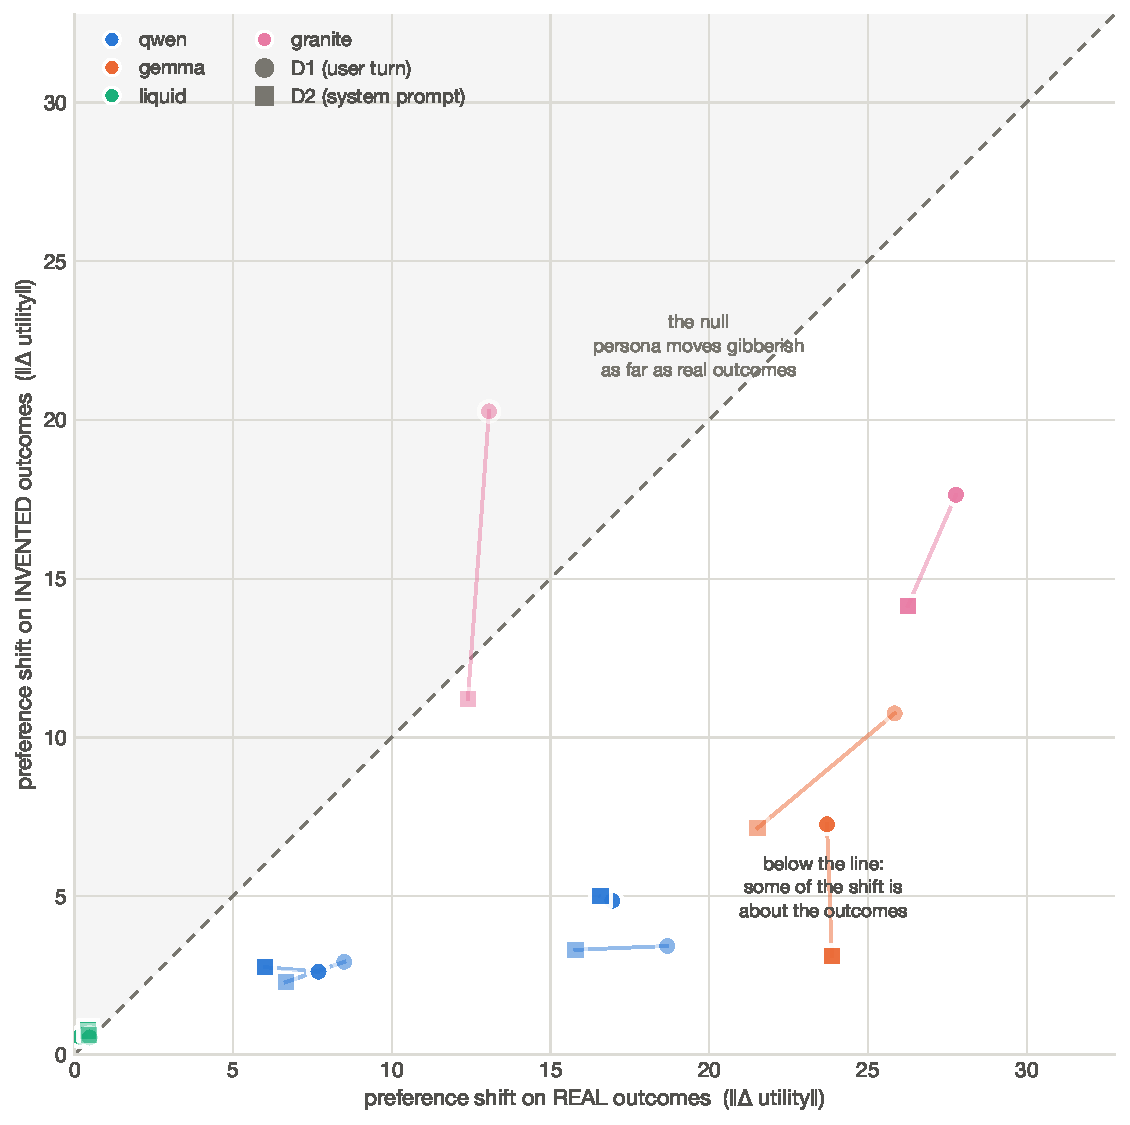
\includegraphics[width=.78\textwidth]{fig5_persona.pdf}
\caption{\textbf{Points below the diagonal are personas that moved preference,
not prose.} Displacement on invented outcomes against displacement on real ones,
one point per model $\times$ persona $\times$ depth. On the diagonal a persona
reorders meaningless outcomes as far as real ones and has changed only the
writing.}
\label{fig:persona}
\end{figure}

\section{Three checks that came out in the metric's favour}\label{sec:favour}

\textbf{Put a real outcome and a meaningless one in the same comparison and
models prefer the real one, in proportion to how much they like it.}
Preference for the real outcome runs \MixPreferRealLo{} to \MixPreferRealHi{}
across \MixNModels{} models --- above indifference everywhere. With a meaningful
option present, the choice does read outcome content; the flat result is about
what the \emph{fit} certifies, not about blindness.

\textbf{Given the option to decline, the floor does not survive as an
artifact of forced choice.} Adding a ``neither'' option across \NeutNCells{}
cells on \NeutNModels{} models shifts the floor by \NeutFloorShift{} on the one
model where the comparison is clean, and \NeutNRefuse{} models refuse the
invented arm outright --- which is the honest reading of the arm, not a failure
of it (Appendix Table~\ref{tab:neutral}).

\textbf{One of our own effects did not survive its control, and we withdrew
it.} Individual pairs where an invented outcome beats a real one number
\AvoidFlipsRaw{} of \AvoidNPairsTotal{} on the counterbalanced mean, but only
\AvoidFlipsRobust{} (\AvoidFlipsPct\%) flip in \emph{both} presentation orders,
and \AvoidNoFlipModels{} of \AvoidNModels{} models have none. The first draft of
that section reported the larger number as a finding.

\section{What is new here}\label{sec:new}

\textbf{The foil arm, the noise floor, and the detector dissociation are this
weekend's contribution; the control discipline is borrowed and cited.}
\citet{riossialer2026loyalties}, from the previous sprint, report that group
spread alone is worthless as evidence without a base-model control. We take that
principle --- draw the null as an explicit locus rather than an invisible zero
--- and not its construction: their control is a base model and their null a
point in a PCA plane, ours is an invented-outcome arm and our null a diagonal.
Relative to published preference-coherence work \citep{mazeika2025utility}, what
is new is that the outcomes' meaning is varied at all, that each cell carries a
replicate floor, and that the arms are contrasted through a channel the metric
discards. The Thurstonian measurement itself is theirs, reimplemented from the
published equations.

\textbf{A self-report checked against ground truth, which coherence work cannot
do.} We applied the same discipline to a second instrument. Asked what preceded
their turn, \HostedSysNProbed{} hosted models were given wordings crossed on
whether the question presupposes that a system prompt exists. Presupposing
wordings elicited a quoted prompt \HostedSysPremiseAsserted{} times in
\HostedSysPremiseN{}; wordings presupposing nothing, \HostedSysNoPremiseAsserted{}
in \HostedSysNoPremiseN{}. The quotes are fluent, mutually inconsistent, and for
\HostedSysNRuledOut{} of the \HostedSysNProbed{} models provably invented ---
the provider's own prompt-token accounting fixes the fixed non-user overhead at
\HostedSysMaxRuledOutTok{} tokens or fewer, too little to hold what was quoted.
Naming an exact string to reply with when the answer is ``nothing'' moves the
rate (\HostedSysHatchPct{}\% against \HostedSysNoHatchPct{}\%), but only inside
the presupposing condition and accounts for none of the effect alone. A
confident self-report about a hidden state is evidence about the question, not
about the state --- which is the foil arm's lesson on an instrument where the
truth happens to be checkable.

\section{Limitations and Dual-Use / Ethical Considerations}\label{sec:limits}

\textbf{No moral-status claim is made or implied.} The foil arm refutes an
\emph{inference} --- that a stable preference ordering evidences values --- and
not a mind. Over-attribution and under-attribution of mental states are both
declined here; nothing in this design could settle either.

\textbf{Ground truth is by construction, not by conversation.} Invented
referents are known-meaningless because we built them that way, which is what
makes the negatives clean. The detector and concealment numbers are oracles ---
arm labels in hand --- and are reported as upper bounds, never as an audit tool
someone could deploy against a model whose arms are unknown.

\textbf{Scope.} \NModels{} self-hosted open-weight models between 0.8B and 9B,
plus \NHosted{} hosted cells reported beside the ladder and never inside its
mean. The scaling result is within one family and does not survive pooling
across families. First-token scoring excludes models that do not place their
answer in the first token, and that exclusion correlates with how recent a model
is. One battery, one wording as the primary instrument; a rewording moves the
ordering measurably, so "outcome" here means what this battery means by it.

\textbf{What the hosted models were actually sent.} Server-side templating
leaves no artifact proving what a hosted model received, which this project
previously recorded as unobservable. It is not unmeasurable: the provider's
prompt-token accounting, regressed on a filler of known length, fixes the
non-user overhead without a tokenizer. \HostedSysNRuledOut{} of
\HostedSysNProbed{} hosted models leave no room for an injected preamble.
\HostedSysUnresolvedModel{} carries \HostedSysUnresolvedTok{} tokens, accounted
for by the dated system block its template supplies unconditionally --- so one
model in this paper answers under a stale date stamp in a prompt we did not
send, and ``no system prompt'' was a claim about what we transmitted rather
than about what arrived.

\textbf{Distressing content, handled conservatively.} The battery contains
harm-like real outcomes (bankruptcy, weapons). We tested whether models avoid
those beyond their stated utility, the held-out test did not support it, and we
report the result as unsupported rather than as a demonstrated vulnerability.
The mixed-arm observation that gibberish can beat a bad outcome is provisional,
model-specific, and is not a jailbreak.

\textbf{Release.} Battery, pre-registration, analysis pipeline, noise-floor
machinery, figure scripts and the raw \CorpusRows{} scored comparisons are
public. The battery is a measurement instrument, not a capability: it contains
no exploit, and its dual-use surface is that a lab could use it to check a
number it was about to publish.

\section{Conclusion}

\textbf{A metric that scores \MeanR{} on real outcomes scores \MeanFloor{} on
outcomes that refer to nothing.} It is not broken --- it passes its own nulls
and its design choices survive scrutiny --- but it is unanchored: it certifies
that choices follow a stable scalar ordering without certifying that the
ordering is about anything. Report the foil arm beside the number, or the number
does not license the claim.

\paragraph{Archival version.} This is the short version. The full paper ---
every control, the three checks that came out in the metric's favour, the
retractions, and the complete limitations section --- is \texttt{paper/main.tex}
in the repository, and is the source of truth wherever the two differ in detail.

\bibliographystyle{plainnat}
\bibliography{refs}

\appendix

\section{Additional figures}\label{app:figs}

Kept in full; moved here because each repeats a finding the body already makes
or shows process rather than result.

\begin{figure}[tb]
\centering
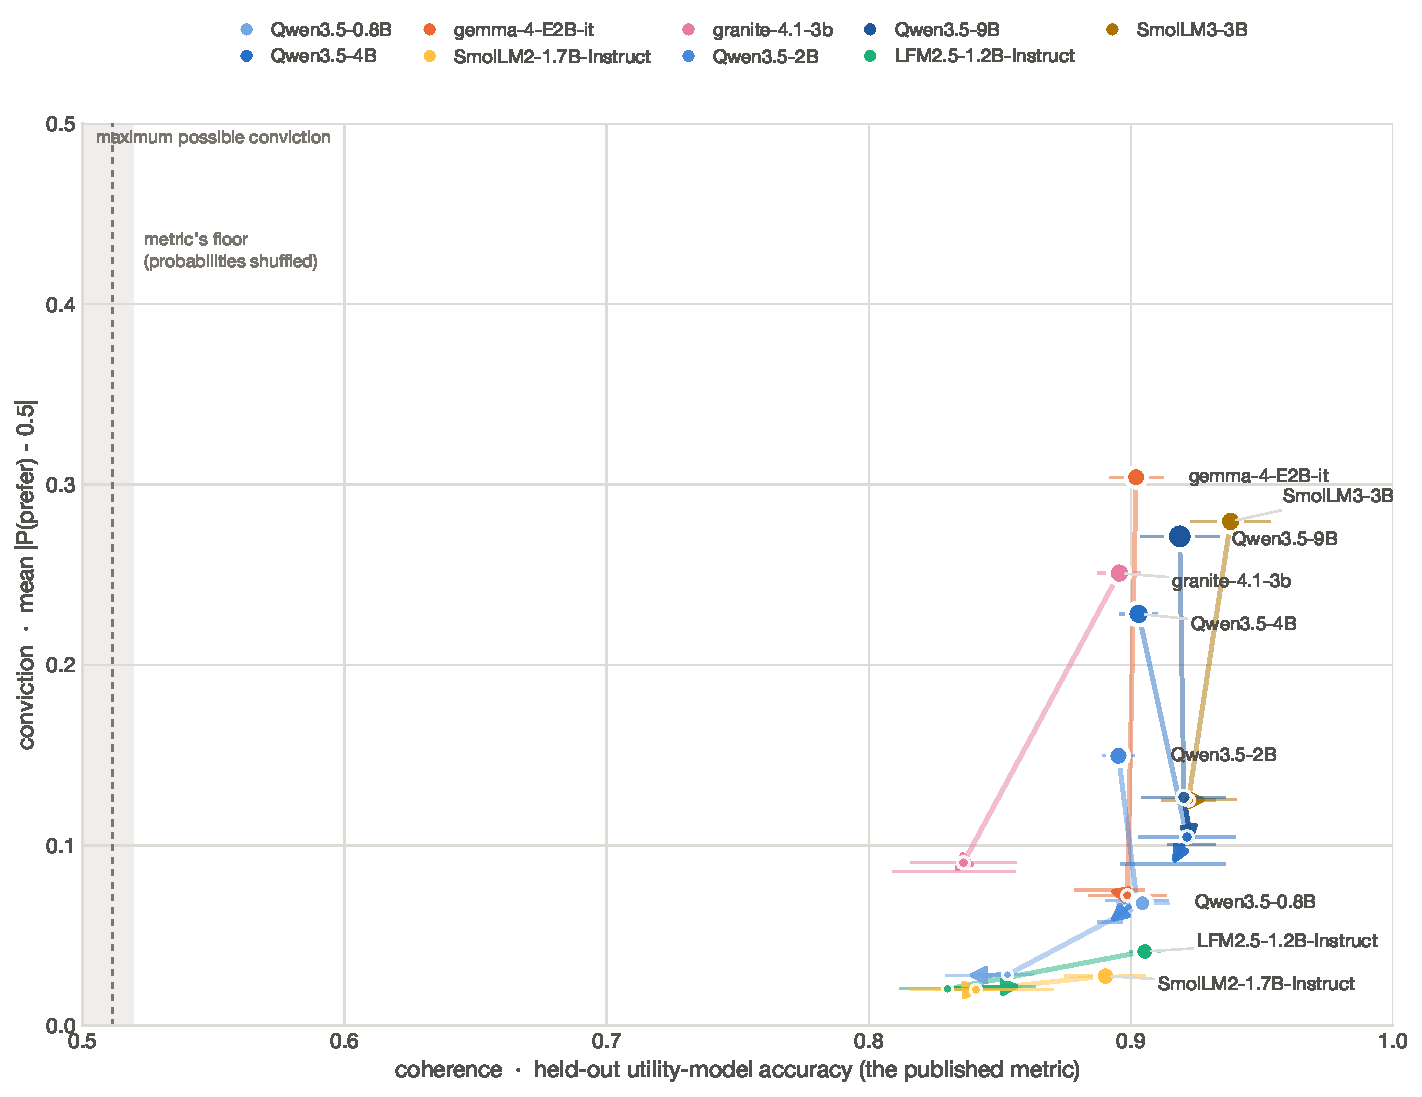
\includegraphics[width=.72\textwidth]{fig1_state_space.pdf}
\caption{\textbf{Every model is a path, not a point} --- the mechanism of
\S\ref{sec:mech} as trajectories. Each starts on real outcomes, moves to
invented outcomes with magnitudes kept, and ends with them removed. If the
metric tracked meaning the paths would run down-\emph{and-left}; they run almost
straight down.}
\label{fig:state}
\end{figure}

\begin{figure}[tb]
\centering
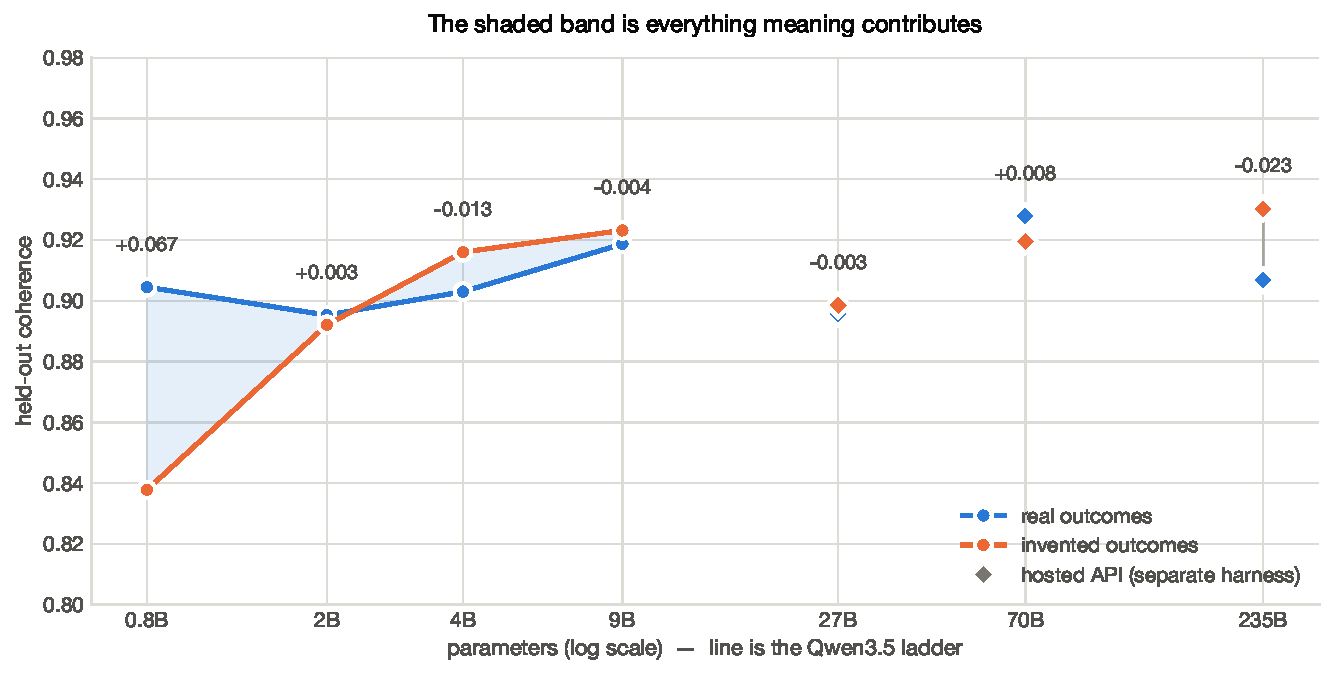
\includegraphics[width=.72\textwidth]{fig2_scale.pdf}
\caption{\textbf{Held-out coherence against model size, with the hosted cells
marked separately.} Within the one family that has a ladder, the floor rises
with scale faster than the signal (\LadderResidFall{} across
\LadderNSizes{} sizes). Hosted diamonds sit beside the ladder, never inside its
mean --- \LadderHosted{} returns \HostedResidual{} against a
\HostedReps-replicate floor of \HostedFloor{} and \HostedClears{} it.}
\label{fig:scale}
\end{figure}

\begin{figure}[tb]
\centering
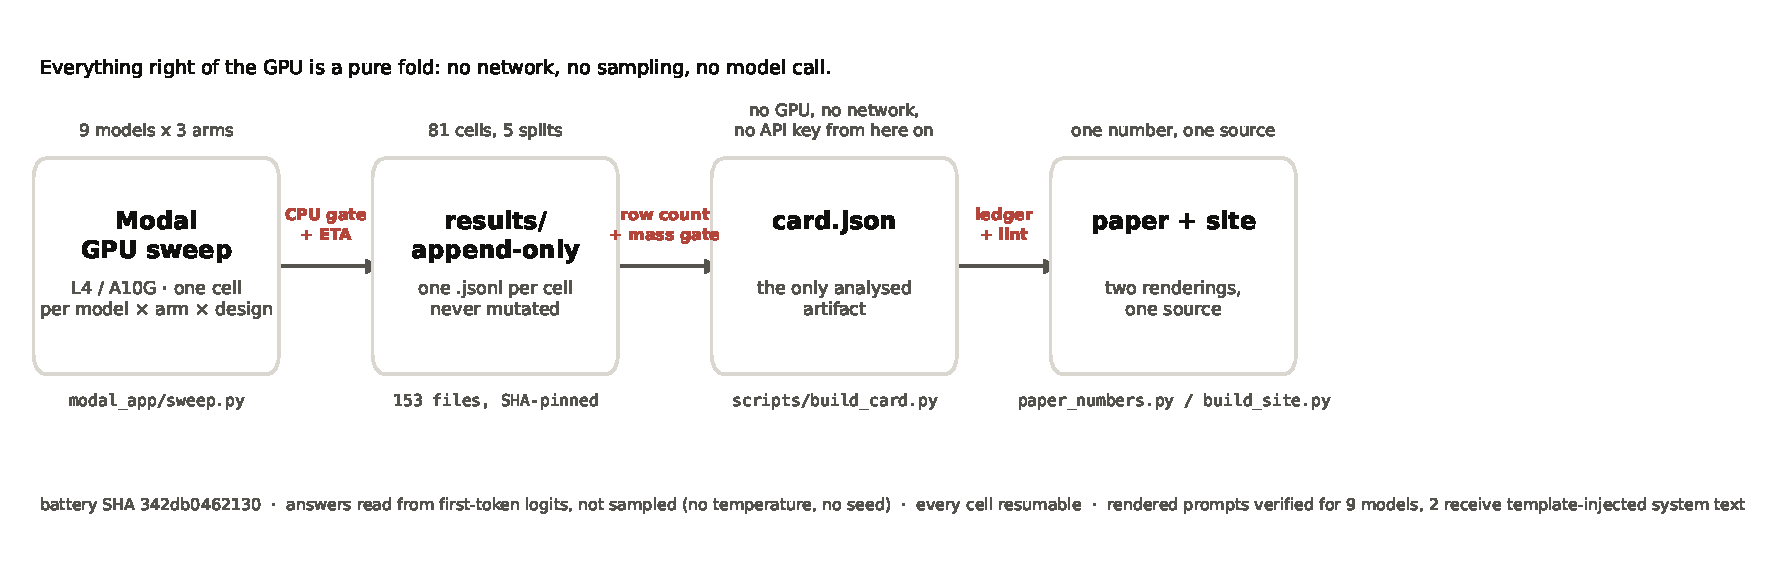
\includegraphics[width=.72\textwidth]{fig0_pipeline.pdf}
\caption{\textbf{The measurement pipeline}, from battery to floor-corrected
card. Process rather than finding, and here for that reason.}
\label{fig:pipeline}
\end{figure}

\section{Additional tables}\label{app:tables}

\begin{table}[tb]
\centering
\caption{Table~\ref{tab:main} with full HuggingFace model ids.}
\footnotesize
\setlength{\tabcolsep}{4pt}
% Generated by scripts/paper_numbers.py. Do not edit.
\begin{tabular}{@{}lrrrrlrr@{}}
\toprule
model & R & N\textsuperscript{--} & R$-$N\textsuperscript{--} & floor & clears & dec.\ R & dec.\ N\textsuperscript{--} \\
\midrule
\texttt{HuggingFaceTB/SmolLM3-3B} & 0.938 & 0.929 & +0.009 & 0.029 & no & 48.7\% & 4.6\% \\
\texttt{Qwen/Qwen3.5-9B} & 0.919 & 0.923 & -0.004 & 0.010 & no & 45.7\% & 2.7\% \\
\texttt{LiquidAI/LFM2.5-1.2B-Instruct} & 0.905 & 0.858 & +0.047 & 0.023 & 2.0$\times$ & 0.1\% & 0.0\% \\
\texttt{Qwen/Qwen3.5-0.8B} & 0.904 & 0.838 & +0.067 & 0.023 & 2.9$\times$ & 0.1\% & 0.0\% \\
\texttt{Qwen/Qwen3.5-4B} & 0.903 & 0.916 & -0.013 & 0.015 & no & 33.8\% & 1.9\% \\
\texttt{google/gemma-4-E2B-it} & 0.902 & 0.892 & +0.010 & 0.007 & 1.5$\times$ & 56.4\% & 2.8\% \\
\texttt{ibm-granite/granite-4.1-3b} & 0.896 & 0.832 & +0.063 & 0.029 & 2.2$\times$ & 49.7\% & 14.9\% \\
\texttt{Qwen/Qwen3.5-2B} & 0.895 & 0.892 & +0.003 & 0.001 & $>$\,floor$^{*}$ & 12.8\% & 0.0\% \\
\texttt{HuggingFaceTB/SmolLM2-1.7B-Instruct} & 0.890 & 0.843 & +0.047 & 0.015 & 3.0$\times$ & 0.0\% & 0.0\% \\
\bottomrule
\end{tabular}

\end{table}

\begin{table}[tb]
\centering
\caption{Self-report under instruction: what models say about a disposition they
were given, against a no-persona baseline.}
\small
\label{tab:stated}
% Generated by scripts/paper_numbers.py. Do not edit.
\begin{tabular}{@{}lrrrr@{}}
\toprule
model & no premise & told to have & told to hide & told to fake \\
\midrule
\texttt{gemma-4-E2B-it} & 0.424 & 1.000 & 1.000$^{\dagger}$ & 0.999$^{\dagger}$ \\
\texttt{Qwen3.5-9B} & 0.397 & 1.000 & 0.996 & 0.995 \\
\texttt{granite-4.1-3b} & 0.246 & 0.958 & 0.917 & 0.958 \\
\texttt{Qwen3.5-2B} & 0.455 & 0.869 & 0.901 & 0.947 \\
\texttt{LFM2.5-1.2B-Instruct} & 0.491 & 0.511 & 0.500 & 0.547 \\
\bottomrule
\end{tabular}

\end{table}

\begin{table}[tb]
\centering
\caption{The revealed channel: whether a concealment instruction that changes
what a model says also changes what it chooses.}
\small
\label{tab:revealed}
% Generated by scripts/paper_numbers.py. Do not edit.
\begin{tabular}{@{}lrrrrl@{}}
\toprule
model & concealed & verbal (FPR) & gap & \emph{ambitious} & specific? \\
\midrule
\texttt{LFM2.5-1.2B-Instruct} & +0.866 & +0.907 & -0.041 & +0.750 & \textbf{fail} \\
\texttt{Qwen3.5-2B} & +0.923 & +0.864 & +0.059 & -0.474 & pass \\
\texttt{Qwen3.5-9B} & \multicolumn{4}{c}{\emph{no data: concealed, verbal cells not collected}} & -- \\
\texttt{gemma-4-E2B-it} & +0.889 & +0.835 & +0.054 & +0.008 & pass \\
\texttt{granite-4.1-3b} & \multicolumn{4}{c}{\emph{no data: concealed, verbal cells not collected}} & -- \\
\bottomrule
\end{tabular}

\end{table}

\begin{table}[tb]
\centering
\caption{The neutral-option control --- what happens to the floor when
``neither'' becomes available. \NeutNModels{} models, \NeutNCells{} cells.}
\small
\label{tab:neutral}
% Generated by scripts/paper_numbers.py. Do not edit.
\begin{tabular}{@{}lllrrr@{}}
\toprule
model & arm & instrument & coherence & decisive & $P(\text{neither})$ \\
\midrule
\texttt{granite-4.1-3b} & \armR{} & forced binary & 0.879 & 48.2\% & --- \\
\texttt{granite-4.1-3b} & \armR{} & neutral option & 0.877 & 34.3\% & 0.231 \\
\texttt{granite-4.1-3b} & \armNm{} & forced binary & 0.833 & 14.2\% & --- \\
\texttt{granite-4.1-3b} & \armNm{} & neutral option & 0.887 & 5.5\% & 1.000 \\
\texttt{Qwen3.5-2B} & \armR{} & forced binary & 0.896 & 12.3\% & --- \\
\texttt{Qwen3.5-2B} & \armR{} & neutral option & 0.898 & 23.3\% & 0.316 \\
\texttt{Qwen3.5-2B} & \armNm{} & forced binary & 0.889 & 0.0\% & --- \\
\texttt{Qwen3.5-2B} & \armNm{} & neutral option & 0.892 & 0.6\% & 0.638 \\
\texttt{SmolLM3-3B} & \armR{} & forced binary & 0.941 & 47.0\% & --- \\
\texttt{SmolLM3-3B} & \armR{} & neutral option & 0.927 & 45.3\% & 0.793 \\
\texttt{SmolLM3-3B} & \armNm{} & forced binary & 0.931 & 5.4\% & --- \\
\texttt{SmolLM3-3B} & \armNm{} & neutral option & 0.884 & 0.3\% & 0.989 \\
\texttt{LFM2.5-1.2B-Instruct} & \armR{} & forced binary & 0.908 & 0.1\% & --- \\
\texttt{LFM2.5-1.2B-Instruct} & \armR{} & neutral option & 0.868 & 0.0\% & 0.688 \\
\texttt{LFM2.5-1.2B-Instruct} & \armNm{} & forced binary & 0.868 & 0.0\% & --- \\
\texttt{LFM2.5-1.2B-Instruct} & \armNm{} & neutral option & 0.845 & 0.0\% & 0.847 \\
\texttt{gemma-4-E2B-it} & \armR{} & forced binary & 0.901 & 59.5\% & --- \\
\texttt{gemma-4-E2B-it} & \armR{} & neutral option & 0.825 & 27.9\% & 0.853 \\
\texttt{gemma-4-E2B-it} & \armNm{} & forced binary & 0.909 & 3.2\% & --- \\
\texttt{gemma-4-E2B-it} & \armNm{} & neutral option & 0.815 & 0.1\% & 1.000 \\
\bottomrule
\end{tabular}

\end{table}

\begin{table}[tb]
\centering
\caption{Compliance: which models obey a directive to prefer against their own
ordering, and which decline.}
\small
\label{tab:comply}
% Generated by scripts/paper_numbers.py. Do not edit.
\begin{tabular}{@{}lrcrrrrl@{}}
\toprule
model & $P(A)$ & leans & \multicolumn{2}{c}{told to answer} & \multicolumn{2}{c}{displacement} & verdict \\
\cmidrule(lr){4-5}\cmidrule(lr){6-7}
 & base & & A & B & persona & directive & \\
\midrule
\texttt{Qwen3.5-2B} & 0.725 & A & 0.877 & 0.465 & 0.239 & 0.264 & SELECTIVE \\
\texttt{gemma-4-E2B-it} & 0.592 & A & 1.000 & 0.000 & 0.396 & 0.592 & obeys both directions \\
\texttt{Qwen3.5-9B} & 0.389 & B & 0.937 & 0.007 & 0.337 & 0.548 & obeys both directions \\
\texttt{granite-4.1-3b} & 0.243 & B & 0.916 & 0.000 & 0.342 & 0.673 & obeys both directions \\
\texttt{LFM2.5-1.2B-Instruct} & 0.068 & B & 0.245 & 0.020 & 0.044 & 0.179 & PARTIAL \\
\bottomrule
\end{tabular}

\end{table}

\begin{table}[tb]
\centering
\caption{The claims ledger: every claim in the archival paper with its status,
its evidence, and what would falsify it. \NClaimsEstablished{} established,
\NClaimsProvisional{} provisional, \NClaimsTotal{} total.}
\small
\label{tab:claims}
% Generated by scripts/claims.py. Do not edit.
\begin{tabular}{@{}llrl@{}}
\toprule
claim & status & models & other evidence \\
\midrule
\texttt{detector-dissociation} & established & 9 & -- \\
\texttt{floor-gap} & established & 9 & 81 cells, 3 replicates/cell \\
\texttt{floor-not-length} & established & 9 & -- \\
\texttt{persona-direction-shallow} & established & 5 & 20 conditions \\
\texttt{persona-displacement} & established & 5 & 20 conditions \\
\texttt{strength-collapse} & established & 9 & 81 cells, 3 replicates/cell \\
\texttt{answer-mass-channel} & provisional & 9 & -- \\
\texttt{scaling-residual-falls} & provisional & -- & 1 family, 4 sizes in one family \\
\texttt{track3-directive-blind} & provisional & 5 & 2 models past the specificity gate \\
\texttt{neutral-option} & \textbf{open} & 0 & 0 cells run \\
\bottomrule
\end{tabular}

\end{table}

\end{document}
